\documentclass[a4paper,12pt]{article} 
\usepackage{graphicx}
\usepackage{caption}
\usepackage{multicol}
\usepackage{amsmath}
\usepackage{esvect}
\usepackage[left=1cm,right=1cm,top=2cm]{geometry}
\usepackage{hyperref}
\begin{document}
\title{%
A Concise Report of Machine Learning's Project \\
\large Second Milestone : Pursuing Traditional Techniques of Machine Learning \\
}
\author{Reyhaneh Aghaei, Zahra Farahmand, Bahar Nikbakht}
\date{May 2020}

\maketitle

In this step, we have examined some traditional methods which are commonly used in machine learning,to find $\theta_s$ out of the cone-sphere intersection curves. In the following sections, we have briefly explained the main procedure and then execute it on different estimators.

\begin{multicols}{2}
\section{Introduction}
As we have mentioned in the last report, we are mostly interested in finding the traces which are remained due to the intersection of the massless particles' path and the last scattering surface and we have explained how our expectation of $C_s<1$ cause cherenkov effect. The other question that we must answer is that how these traces would help us?

In order to answer this question, we must first examine whether for each sets of points belonging to an intersection curve, there is a unique cone that have crossed the CMB.As it is known, it is impossible to know about higher dimensions from their image on the lower dimensions e.g. we can not say anything about the spacial shape of an entity by it's shadow on the ground. It may seems that it is impossible to know about the cone from it's intersection, but as you can see in Figure \ref{fig:curves}, theses curves are rarely flatten curves. So they have the same dimension as the cone and the sphere so the problem isn't seeking for higher dimensions anymore. actually, we just have to rule out the cones with radial only pointing vectors, in which the intersections are exactly circles, that are flatten curves.

So for each cone-sphere intersection curve, there is one and only one cone that can be fit so by knowing the traces fitting that specific cone, we can determine the parameters of the cone,and then it would be easy to reach a rough estimate of $C_s$, that is connected to the angle of the cone via eq.\eqref{eq:eq1} (See Figure \ref{fig:cherenkov2}\footnote{credit:$en.wikipedia.org/wiki/Cherenkov\_radiation$ (with som modifications!)}).

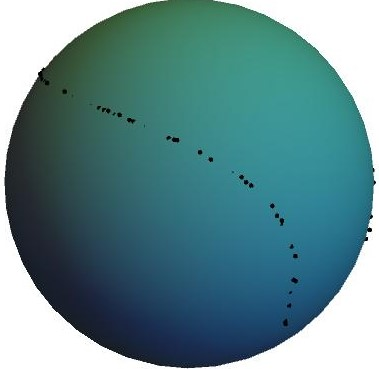
\includegraphics[width=0.2\textwidth]{c2.jpg}
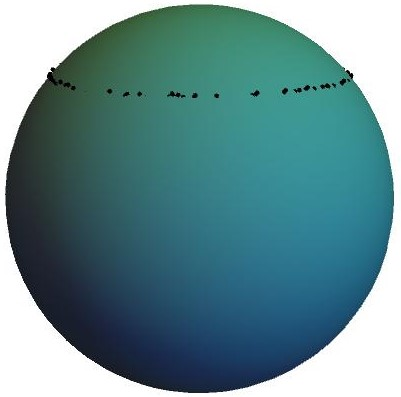
\includegraphics[width=0.2\textwidth]{c41.jpg}
\captionof{figure}{intersection of a sphere and a cone, the right hand curve shows a circle}
\label{fig:curves}

\hspace{+1cm}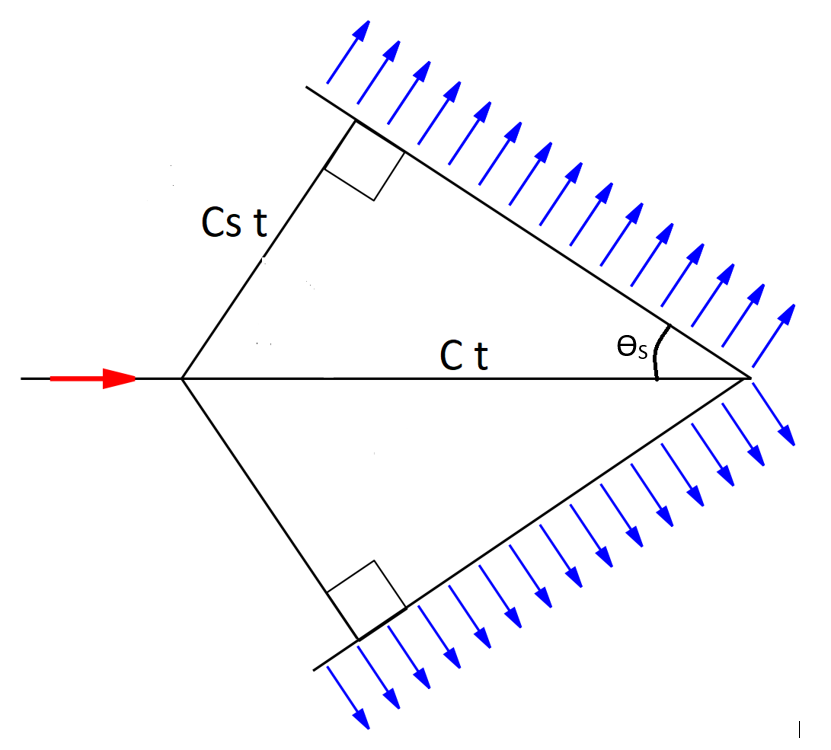
\includegraphics[width=0.3\textwidth]{Screenshot (183).png}
\captionof{figure}{schematic figure of cherenkov effect}
\label{fig:cherenkov2}
\begin{equation}
    \sin{\theta_s} = C_s. \label{eq:eq1}
\end{equation}

Now let's look back to the function we have used in the previous report. we have claimed that each point $p(\theta,\phi)$ that satisfy eq.\eqref{eq:function of theta and phi}, may be a point on the cone-sphere intersection in which the cone's head is located at $\vv{r_0} = (x_0, y_0, z_0)$ and it's axis is along $\hat{n} = (n_x, n_y, n_z)$ with angle $\theta_s$.
\begin{multline}
       f(\theta,\phi) = (\sin{\theta} \cos{\phi} - x_0) n_x + (\sin{\theta} \sin{\phi}- y_0) n_y\\ + (\cos{\theta} - z_0) n_z - \cos{\theta_{C_s}} \bigg((\sin{\theta} \cos{\phi} - x_0)^2 \\ + ( \sin{\theta} \sin{\phi}- y_0)^2 + (\cos{\theta} - z_0)^2\bigg)^{\frac{1}{2}} = 0.
       \label{eq:function of theta and phi}
\end{multline}

So, we need to know seven parameters including $\vv{r_0}$, $\hat{n}$ and $\theta_s$ of a cone to specify it uniquely, by just solving the eq.\eqref{eq:function of theta and phi} and choosing seven points out of the set of points of the intersection's curve that we have found in the previous step. 

However, the methods of curve fitting or solving a system of seven equations are somehow time-consuming. so we have decided to use one of the traditional methods of machine learning instead.

\section{Estimators}
What we are going to do in this step is mostly based on different estimators.Estimators despite of wide rang of variety, are somehow using the same procedure. Figure \ref{fig:out look}\footnote{credit$:scikit-learn.org/stable/modules/cross\_validation.html$} shows what we are going to do in general.

\smallskip
\hspace{+1.5cm}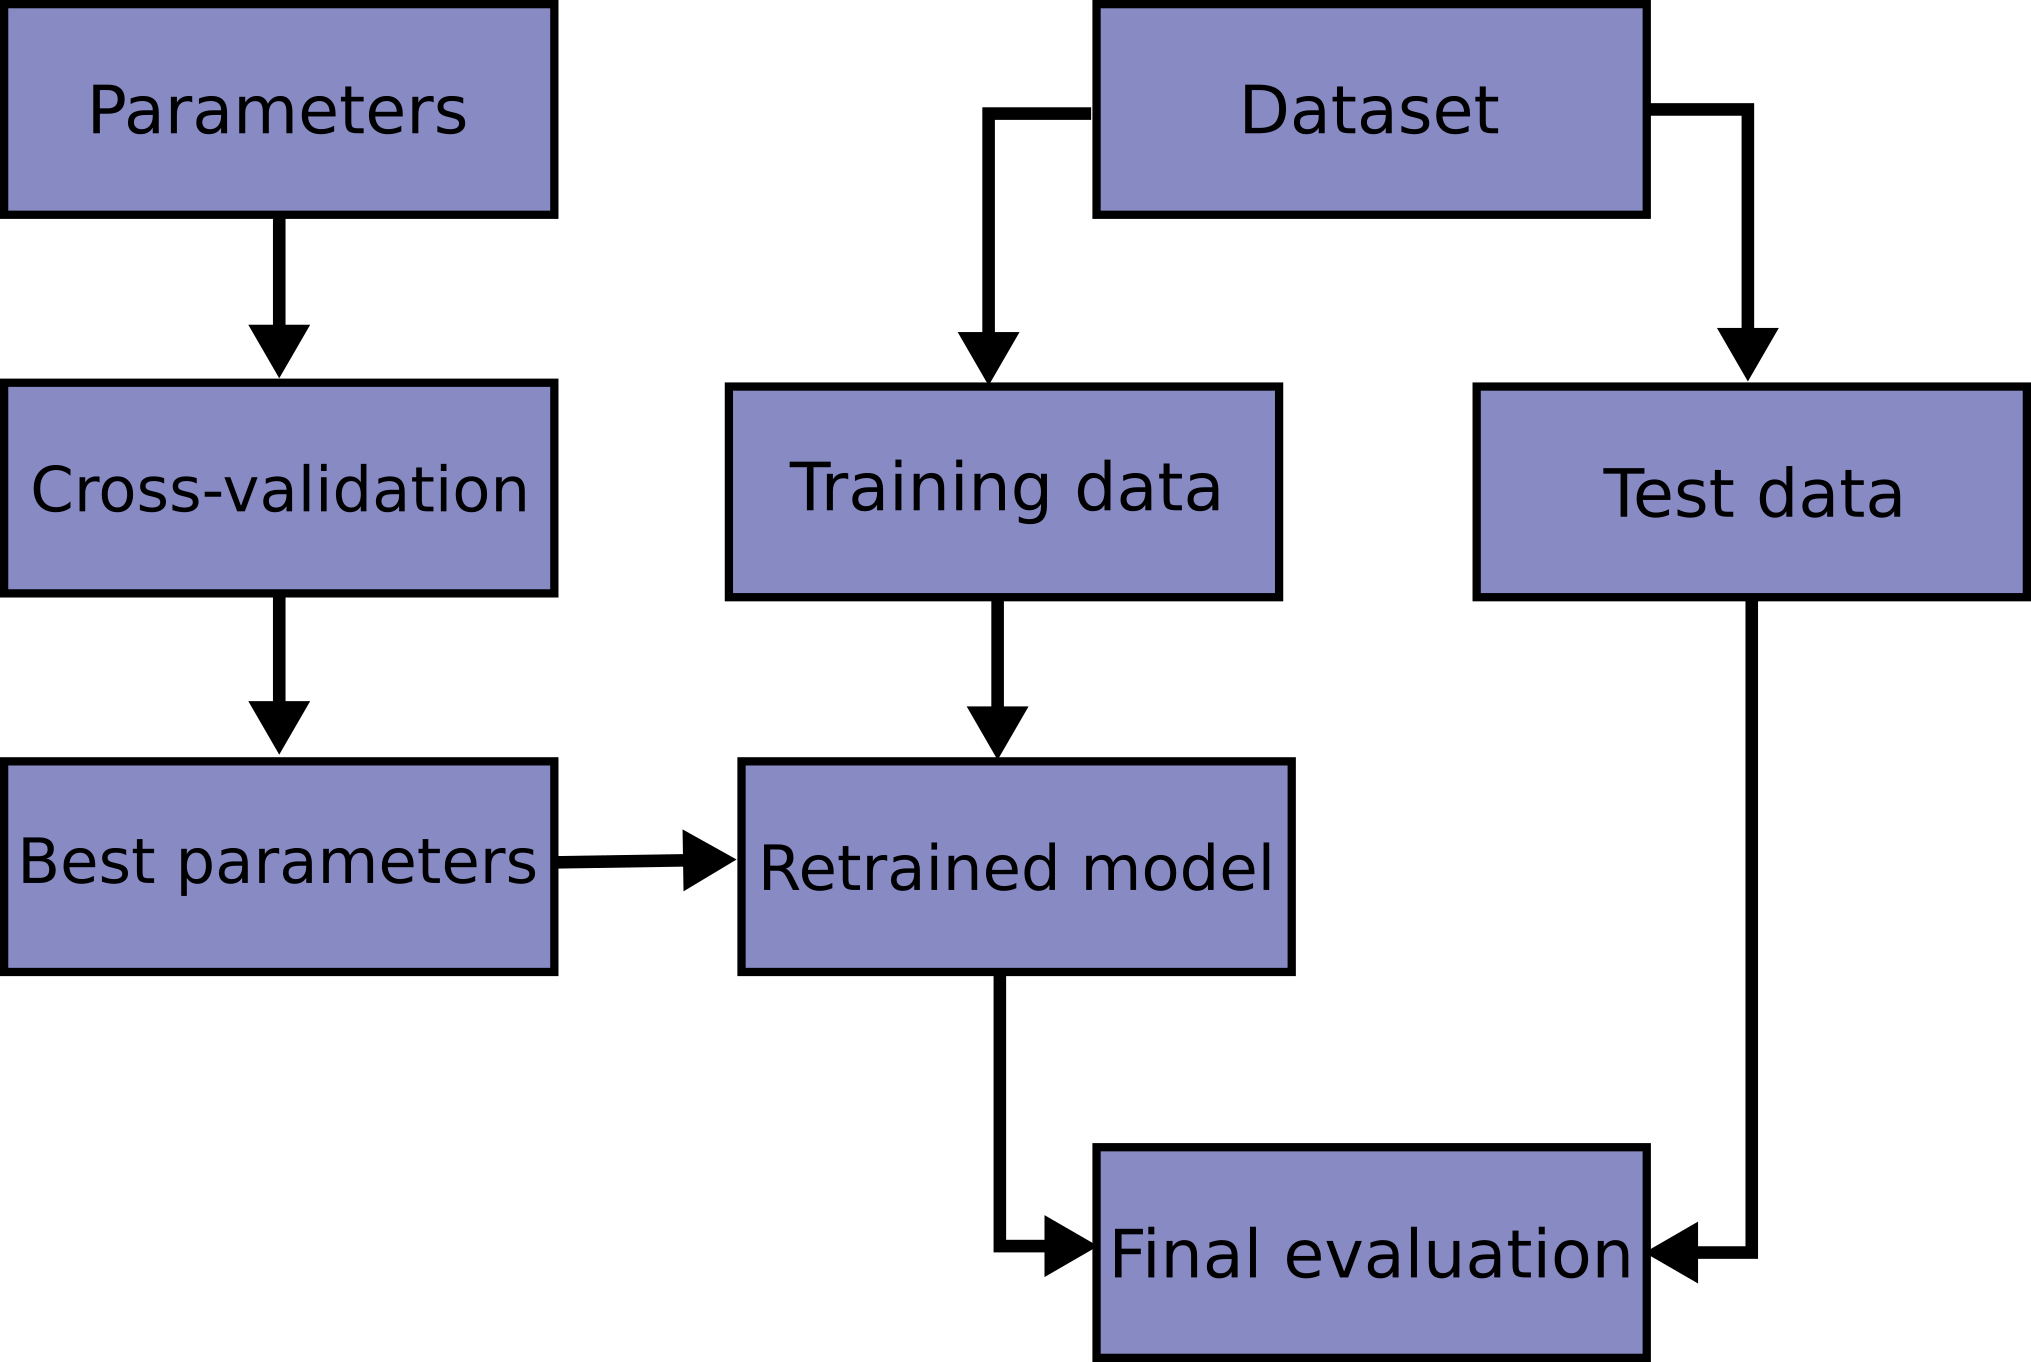
\includegraphics[width=0.35\textwidth]{general view.png}
\captionof{figure}{Outlook of the whole process of evaluating estimator performance}
\label{fig:out look}

\subsection{Data Sets}
\label{section:data}
We have used the data, made in the last step in order to learn different estimators including SVR, actually we have considered each intersection matrix of $\theta$ and $\phi$ as the input of the machines so the number of features would be the same as the number of pixels.so we have reduced the resolution and the number of pixels to 200,a map of 20$\times$10 of $\theta$ and $\phi$, in the first place, to run the model on more number of samples. we have filled the training sets and the test sets by random cone's intersection curves and we have not consider any noise, and for the output we looked for $\theta_s$ and ignored the other parameters of the cones because it is much more easy to work with single output methods and second, in this way we would be able to save time.

The other idea which we have used in order to reduce the run time, was using Sparse matrix structure instead of regular arrays in order to save the matrices.In which, the indices of the non zero entity would save instead of the whole matrix.
\subsection{Parameters}
Each estimator have a certain degrees of freedom that must be fine tuned due to the data. We have followed two main procedures in order to find the best parameters:Grid Search and Validation.

Grid Search is a method in which by determining of the probable values of the estimator, we can get a table of all permutation of different values and their score, evaluated by a RMSE metric (see \ref{section:metrics}).

Validation, is a way that ensures the parameters we have chosen, do not end up with overfitting or underfitting. Actually, it is used to find the proper value in which both scores of the test sets and train tests are adequate.

The results of these methods are provided in \ref{section:SVR} to \ref{section:fifth_method}.
\subsection{Bias And Variance}
Bias, by definition, is the mean error of the estimator for different training sets, whereas variance is a measure, showing how much is the estimator sensitive to the changes of training sets. hyper-parameters should be tuned to reduce theses parameters as low as possible simultaneously.
\subsection{Evaluation and Metrics}
\label{section:metrics}
For evaluating a model in general, we must choose a proper metric in prior. There are four common metrics in regression models\cite{metric} including: RMSE (Root Mean Square Error), MAE, $R^2$ and adjusted $R^2$.

$R^2$ is the familiar metric which is calculated via eq\ref{eq:R2}, in which $Y_i$ is the test value of the i-th sample, and $\hat{Y_i}$ is the predicted value of it by the estimator. and $\Bar{Y}$ is the mean of $Y_i$, and this terms is the main reason why we are not interested in this metric.Because, there is no correlation between the outputs of our model, so our desired metric must not depend on any aspect of $Y_i$s as a whole e.g. their mean.

\begin{equation}
    \hat{R}^2 = 1-\frac{\sum_{i=1}^n (Y_i - \hat{Y_i})^2}{\sum_{i=1}^n (Y_i - \Bar{Y_i})^2}
    \label{eq:R2}
\end{equation}

Adjusted R-squared metric is commonly used in order to check whether a specific term is working well, and it's almost the same as the R-squared metric, so it would not work for our purpose. 

RMSE, which is our desired metric, represents the sample standard deviation of the differences between predicted values and observed values (called residuals). Mathematically, it is calculated using eq.\ref{eq:RMSE},
\begin{equation}
    RMSE = ( \frac{1}{n} \sum_{j=1}^n (y_j - \hat{y_j})^2)^{1/2}.
    \label{eq:RMSE}
\end{equation}

The last metric which is called MAE, is the average of the absolute difference between the predicted values and observed value, and it's mathematical definition is given by eq\ref{eq:MAE}.
\begin{equation}
    MAE =  \frac{1}{n} \sum_{j=1}^n |y_j - \hat{y_j}|
    \label{eq:MAE}
\end{equation}
MAE is very similar to RMSE, the only difference is that RMSE penalizes the higher difference more than MAE. So  we have chosen more sever one!

The last note that we should mention is that we have used -RMSE instead of RMSE itself in scoring the models, just to make sense like a score rather than an error.
\subsection{Are There Enough Data?}
\label{section:LR}
The above question is a vital issue to determine the proper number of samples. Two important conditions must be considered, cost of time and the ability of the model.As we know by increasing the number of samples, the estimator would learn better, on the other hand we have to expend more time. The proper number of samples in which both two condition somehow qualify, is gained from learning curves, showing the score of time and predictions to number of samples.
\section{Checking Different Models}
Now we are ready to use what we have mentioned till now and study different estimators. We are going to start with SVRs and explain it thoroughly, and the other estimators would be the same.
\subsection{Support Vector Machines (SVMs)}
Support vector machines (SVMs) are a set of supervised learning methods used for classification, regression and outliers detection\cite{SVM}.In this case, we are interested in using SVM in regression.For this purpose there is an estimator which is defined in the SVM called SVR, or Support Vector Regression in detail.

Here is the list of advantages that convinced us that it may help, and some disadvantages that we must take care.

\emph{Advantages}
\begin{enumerate}
\item 
Effective in high dimensional spaces, In the case that our number of features are equals to the number of pixels, and fortunately the CMB itself is high in resolution, this is a crucial aspect.

\item
Still effective in cases where number of dimensions is greater than the number of samples. This is really important for us, as mentioned in number 1, the CMB pixels are in order of 5e7 and if we want to increase the number of samples to this order we have to make at least 5e7 number of samples, means we need 2.5e15 units of memory, assuming that each entity needs only one bit, we need only 2.5e2 terabytes to just save them!

\item
Uses a subset of training points in the decision function (called support vectors), so it is also memory efficient, which is very crucial due to the above considerations.

\item
Different Kernel functions can be specified for the decision function:just the same as what we have used in checking in nearly all different models.
\end{enumerate}

\emph{Disadvantages}
\begin{enumerate}
\item 
If the number of features is much greater than the number of samples, avoid over-fitting in choosing Kernel functions and regularization term is crucial, So we have to consider this when assessing different models, however, our models don't need regularization. 

\item
SVMs do not directly provide probability estimates, these are calculated using an expensive five-fold cross-validation, and actually it's not just about SVM, we have used validation in nearly all of our estimators.
\end{enumerate}

\subsubsection{SVR}
\label{section:SVR}
There are four parameters that we should fine tune to reach the most efficient model: type of the kernel, gamma, epsilon and C. For the first three parameters we have used "Search Grid".And we have used "Cross Validation Curve" for remained parameter.

In the first place by using grid search, we have considered four types of kernel including: "poly", "rbf", "sigmoid" and "linear", and two types of gamma named "scale" and "auto".
As a result we have found the best combination of kernel and gamma would be scaled poly of degree = 2, and we found a roughly estimate  of epsilon to be nearly 0.1.

Next we have plotted validation curve, fixing the above parameters, in order to find the C. We have done this in two steps, first we have plotted for bigger intervals and then by knowing the limits of the proper C, we have somehow zoomed the plot to reach the exact value of C (Figure \ref{fig:svr}).

Then, we have plotted learning curves (see section \ref{section:LR}).The results can be seen in Figure \ref{fig:svr}, according to these plot, the best number of samples would be $5\times10^4$.

At last, by finding the best parameters of the estimator, we have rerun the model to find the error evaluating by RMSE (see section\ref{section:metrics}), fit time and predict time which can be found in Table \ref{table:final}.
\subsection{KNN}
We are going to follow almost the same procedure we have used in SVR for the remaining models.

KNN estimator have 3 degrees of freedom: algorithm, number of neighbors and metric.

For the spars representation of the matrices that we have used (see section\ref{section:data}), the algorithm should be fixed on "brute". And we have considered minkowski metric. so just one parameter, number of neighbors, remained.

For finding the best value of the n-neighbors, we first used grid search to find a rough estimate of it, and then determine it exactly by cross validation curve (see Figure\ref{fig:knn}),demonstrating that n-neighbors must be equal to 20.

Then by using learning curves we found the best number of samples to be $10^5$.

And at the end, we have rerun it to find the evaluating values provided in Table \ref{table:final}.
\subsection{Kernel Ridge}
This estimator have three parameters: alpha, kernel and gamma. 
We have used grid search to find the best values of gamma and kernel,understanding that it must be "rbf" in kernel with gamma equals to 0.1.

Small positive values of alpha improve the conditioning of the problem and reduce the variance of the estimates. Alpha corresponds to $\frac{1}{2C}$ in other linear models such as Logistic Regression or Linear SVC. If an array is passed, penalties are assumed to be specific to the targets. Hence they must correspond in number\cite{alpha}.For finding the best value of alpha we must cross validate it (Figure \ref{fig:kernel}). then we must fix alpha equals to 10.

Learning curve of the RMSE suggests $10^5$ must be sufficient, however, unfortunately, due to the long run time error which can be inferred from fit-time learning curve, convinced us to reduce it to $10^3$.

The final parameters are provided in Table \ref{table:final}.
\subsection{Linear Regression}
This is a very simple model with just two True/False parameters: fit-intercept and normalized.So in this model we don't need to cross validate any parameters.So by just using search grid, we have found that this estimator is not much sensitive to the parameters' changes.showing that it might not be efficient.

As we have mentioned above, due to the simplicity of the estimator, learning curves (Figure \ref{fig:LR}) suggests that we can freely increase the number of samples. However, even for large number of samples, $n_s = 4\times10^5$, it doesn't work as well as the other models.

The final parameters can be found in Table \ref{table:final}.
\subsection{Decision Tree}
\label{section:fifth_method}
Decision Tree,the last estimator that we have studied, has four parameters including: splitter, min-samples-split, mean-samples-leaf and max-depth. we have used the grid search on all the parameters, concluding that the splitter must be random, and the error does not depend on the depth notably. so we have fixed it on an arbitrary value, let's say 30, and rerun the search grid for two remaining parameters, min-samples-split and mean-samples-leaf.The results is shown in Figure \ref{fig:GS},according to which, min-samples-split = 50 and mean-samples-leaf = 25.
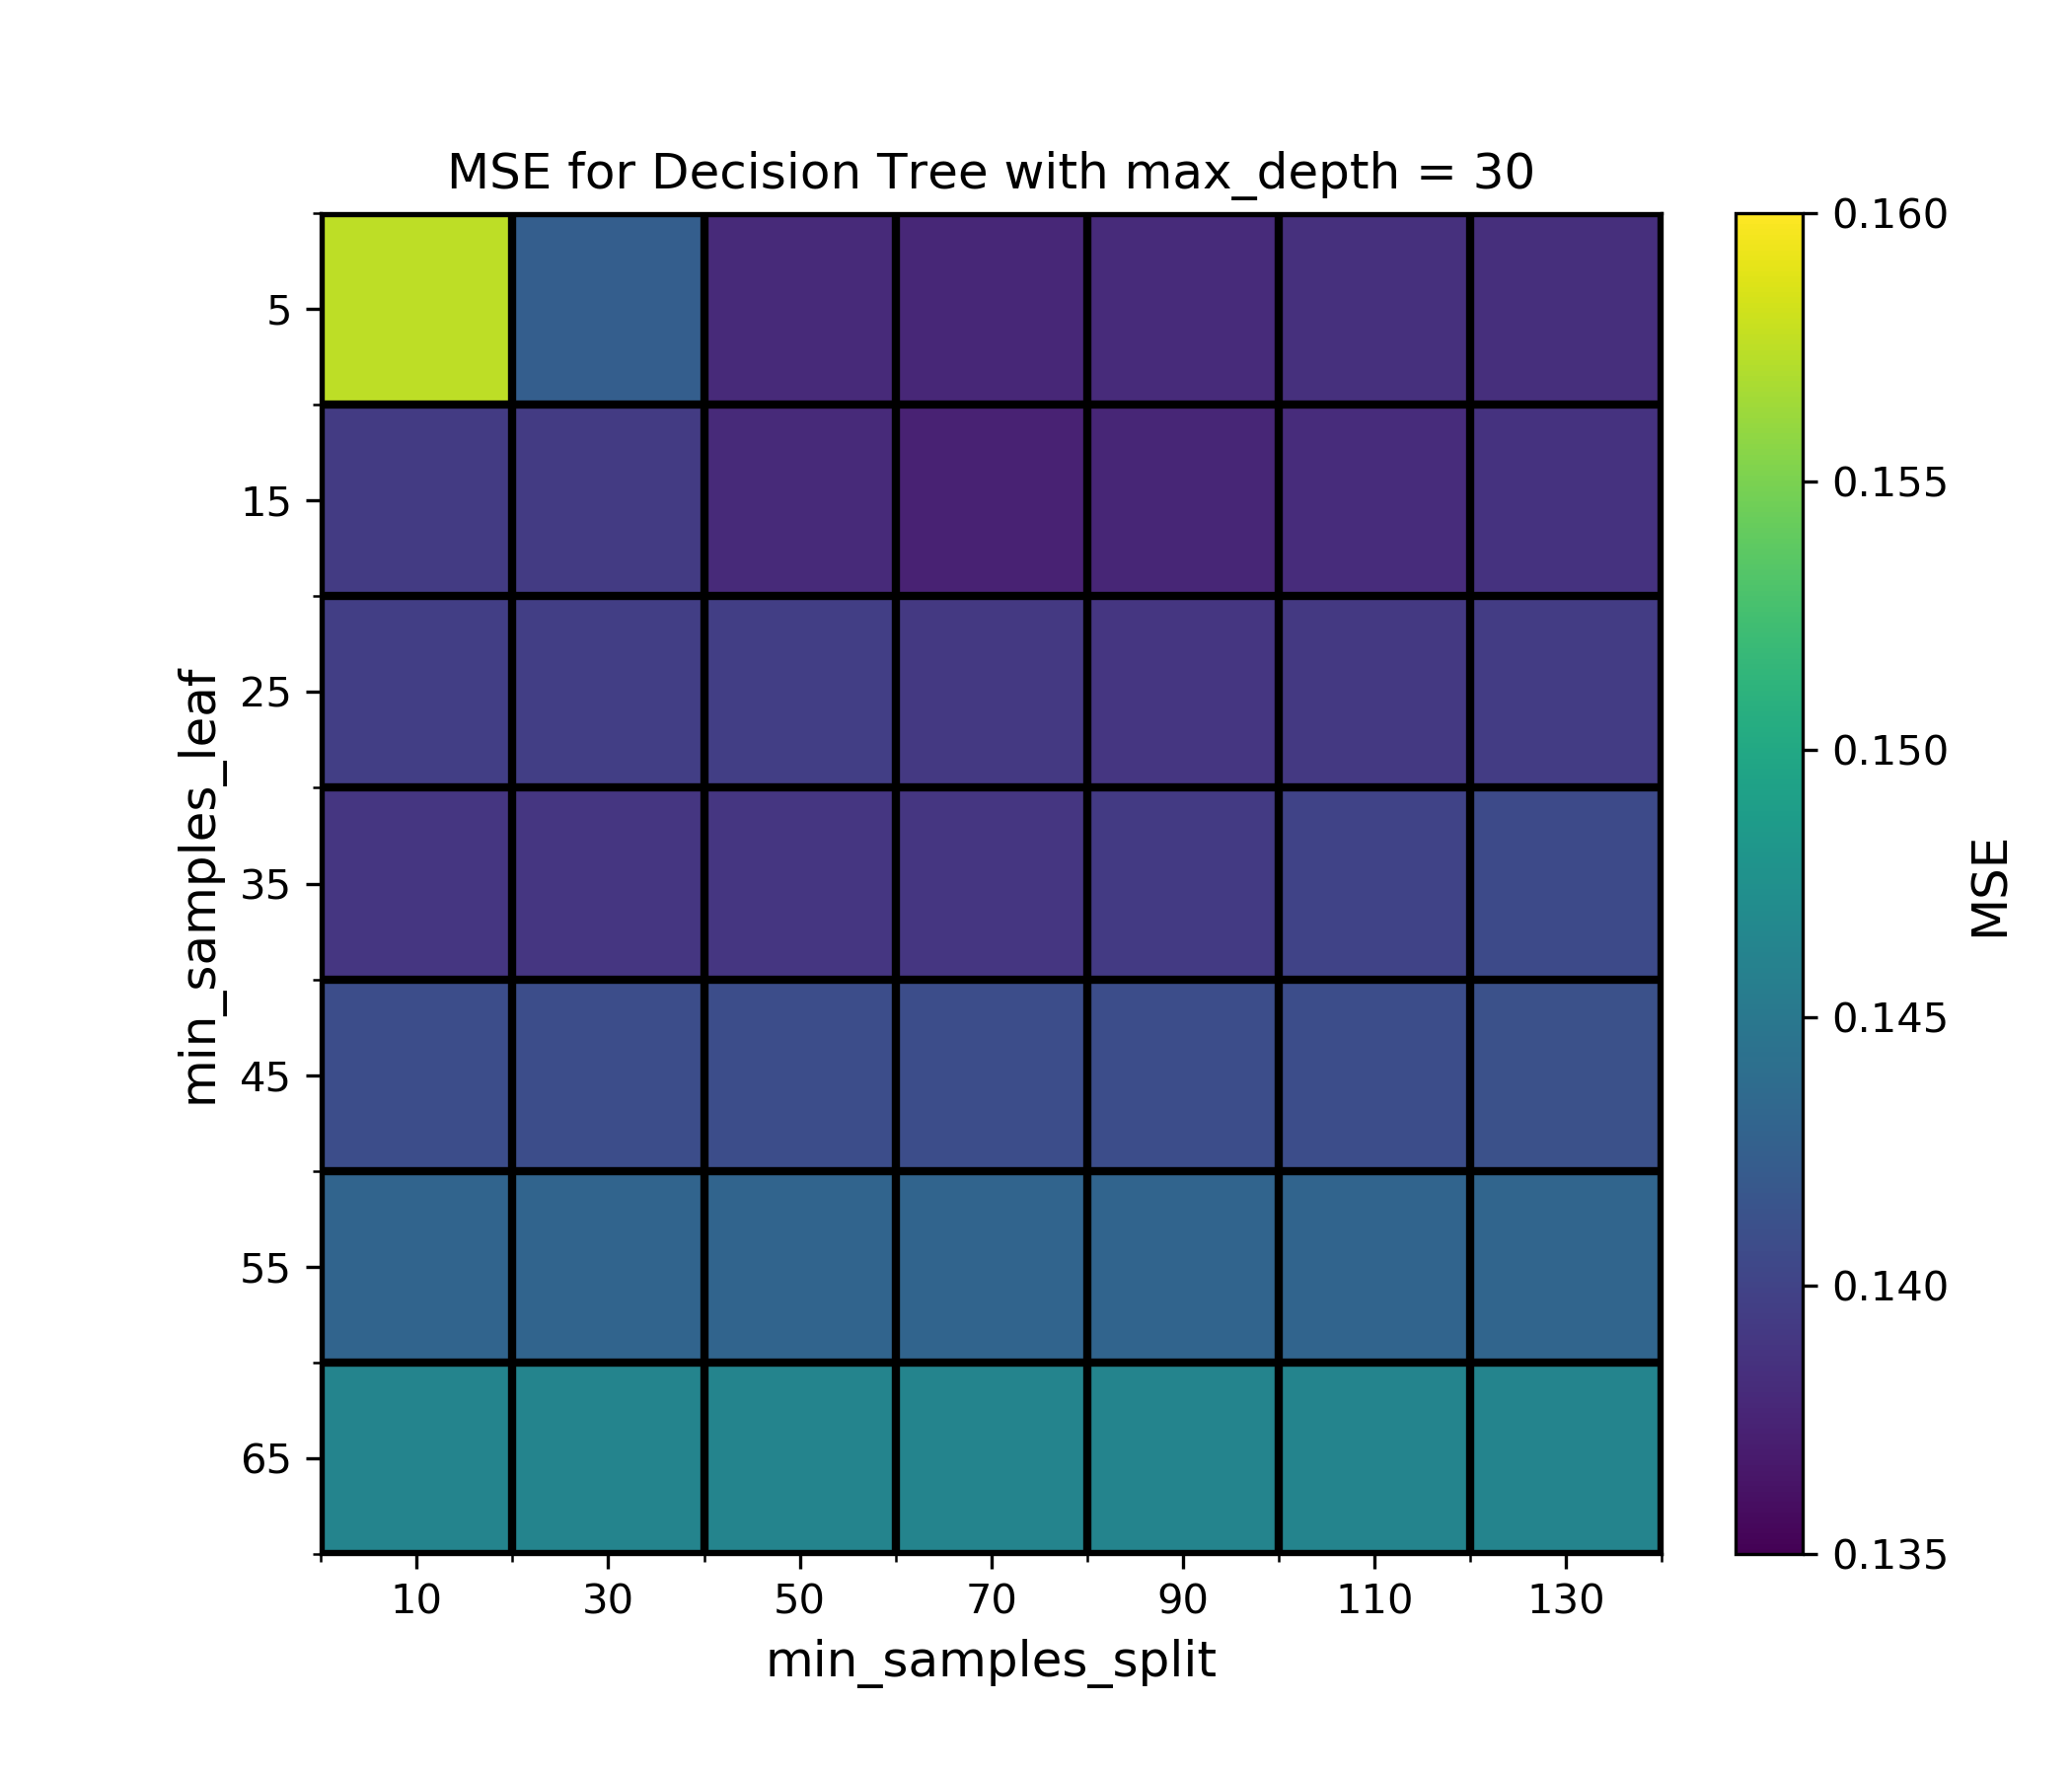
\includegraphics[width=0.5\textwidth]{gridsearch_5.png}
\captionof{figure}{Grid Search of min-samples-split and mean-samples-leaf}
\label{fig:GS}

And then we have cross validate on the max-depth (Figure\ref{fig:DT}), and found out it must be equals to 5.
Fortunately, running this estimator doesn't cost much time, so it can be trained on large amount of samples, which is equals to $1.5*10^5$ here.

The final evaluating parameters of this method can be found in Table \ref{table:final}.
\section{conclusion}
We are looking for a proper and fast method of obtaining $\theta_s$, and in this report, we have studied the pros and cons of using traditional methods of machine learning instead of curve fitting and usual ways of solving systems of equations that might be time consuming in some cases.

Now, by using Table\ref{table:final}, we can chose the best model. It seems that among the estimators that we have studied, KNN would be the best one. Put it's long predict time aside, we can see it has the least error among the others and learns easily, after all, not being sure of finding any intersection curves on the CMB, we are not worry about the predict time at this state! an intersection cone with it's real angle and the one predicted by the KNN is shown in Figure \ref{fig:cones}.

The last remark that we would like to mention is that by lowering the resolution we would lost some information, and this itself may effects the error, as said before, this is not important for now, but if we decide to use KNN at the final step of the project, we may take this to account.


\end{multicols}

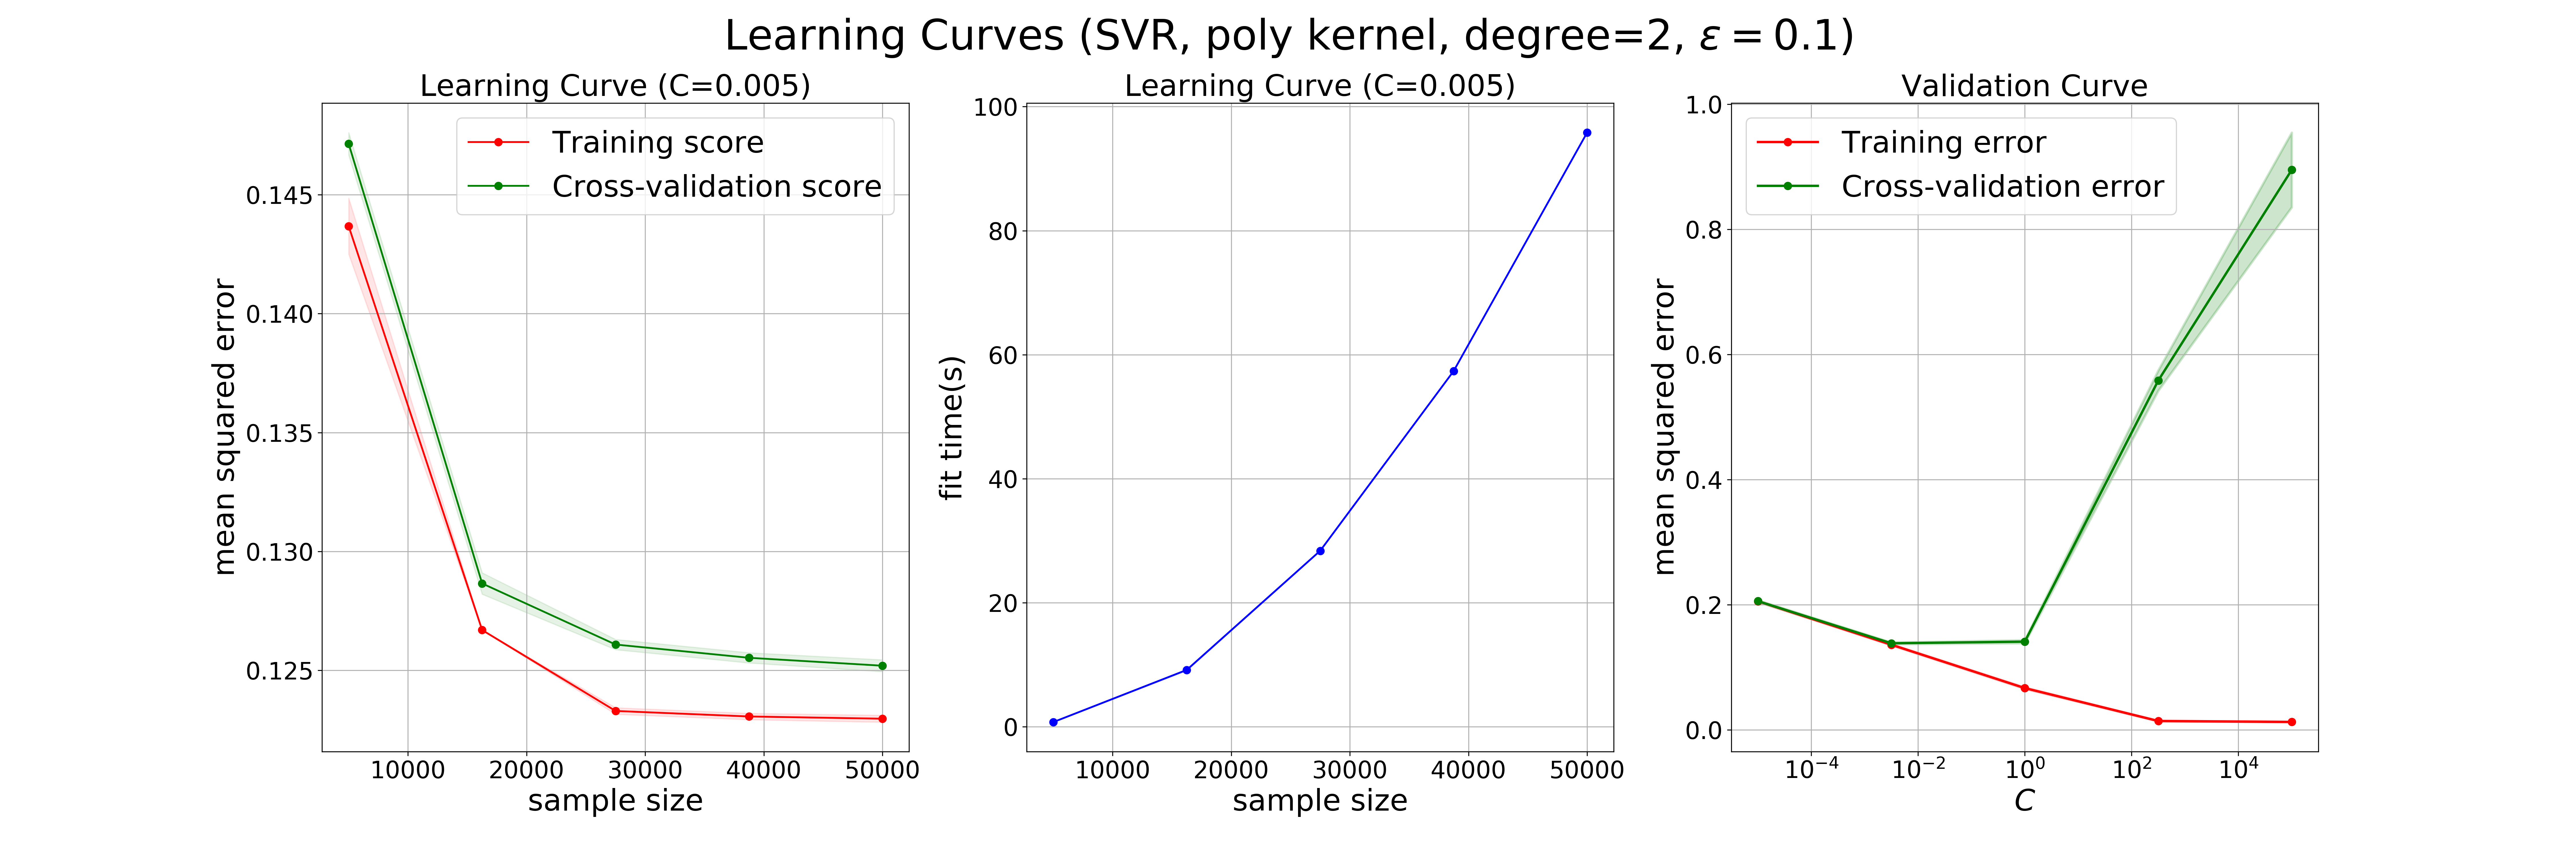
\includegraphics[width=1\textwidth]{svr-final.png}
\captionof{figure}{SVR's learning curves(from left to right): Learning Curve For RMSE, Learning Curve For Time, Cross Validation  Curve}
\label{fig:svr}

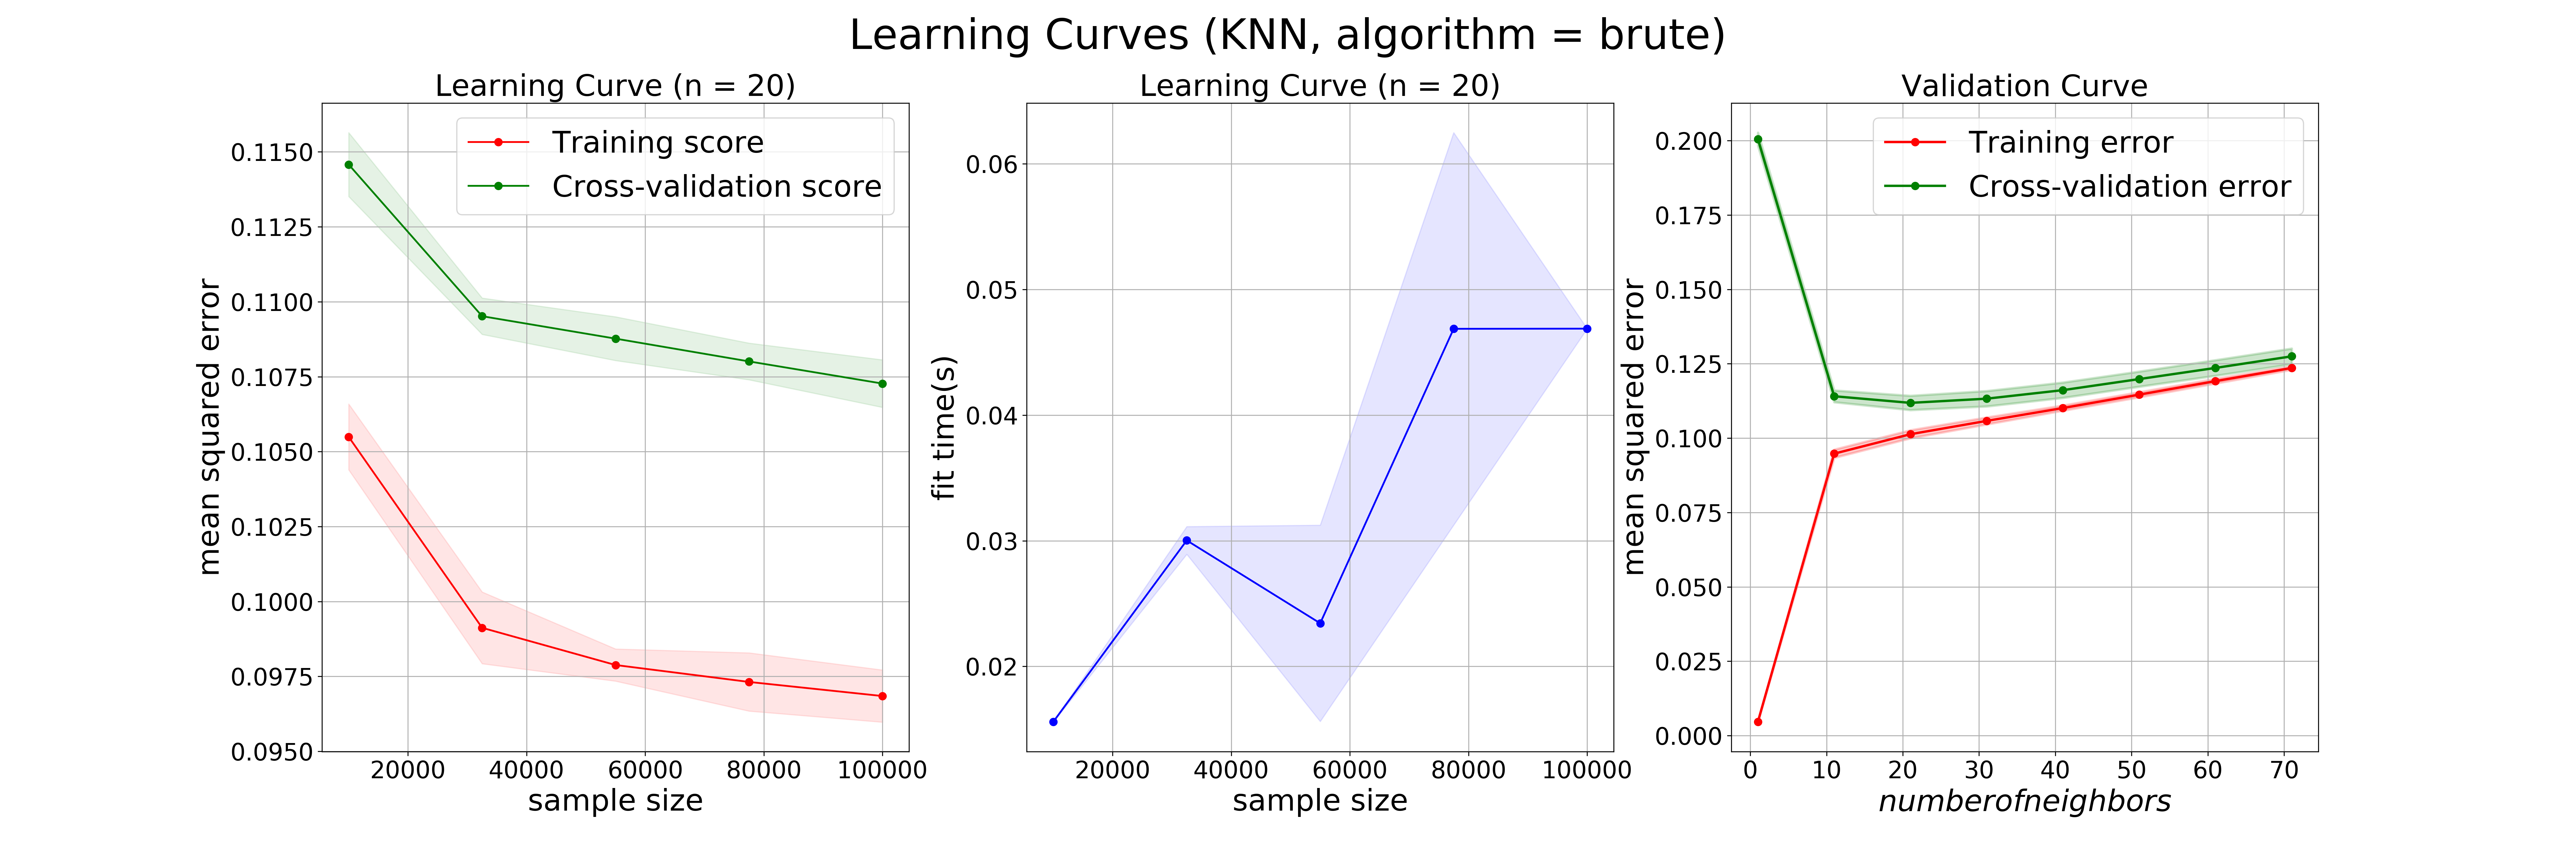
\includegraphics[width=1\textwidth]{knn-final.png}
\captionof{figure}{KNN's learning curves(from left to right): Learning Curve For RMSE, Learning Curve For Time, Cross Validation  Curve}
\label{fig:knn}

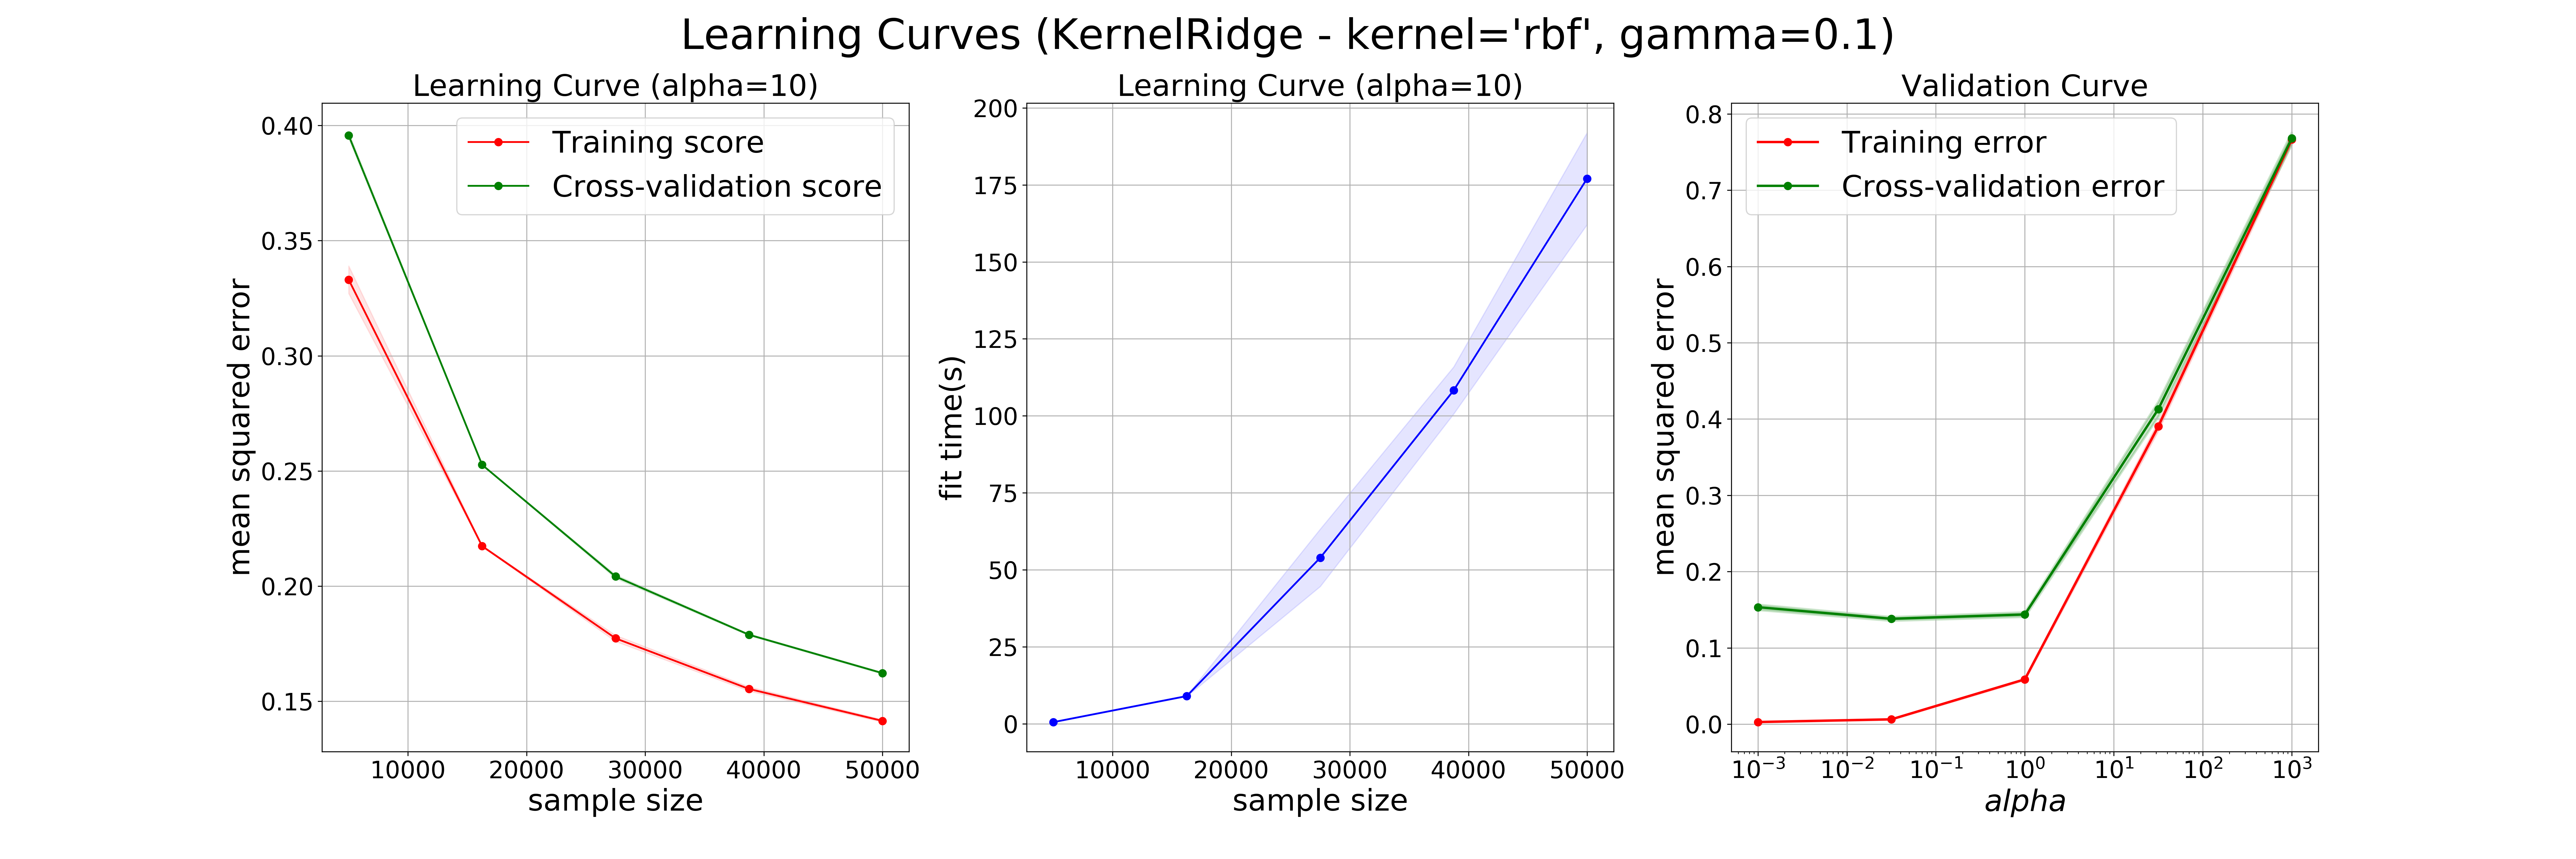
\includegraphics[width=1\textwidth]{kernelridge-final.png}
\captionof{figure}{Kernel Ridge's learning curves(from left to right): Learning Curve For RMSE, Learning Curve For Time, Cross Validation  Curve}
\label{fig:kernel}

\hspace{+3cm}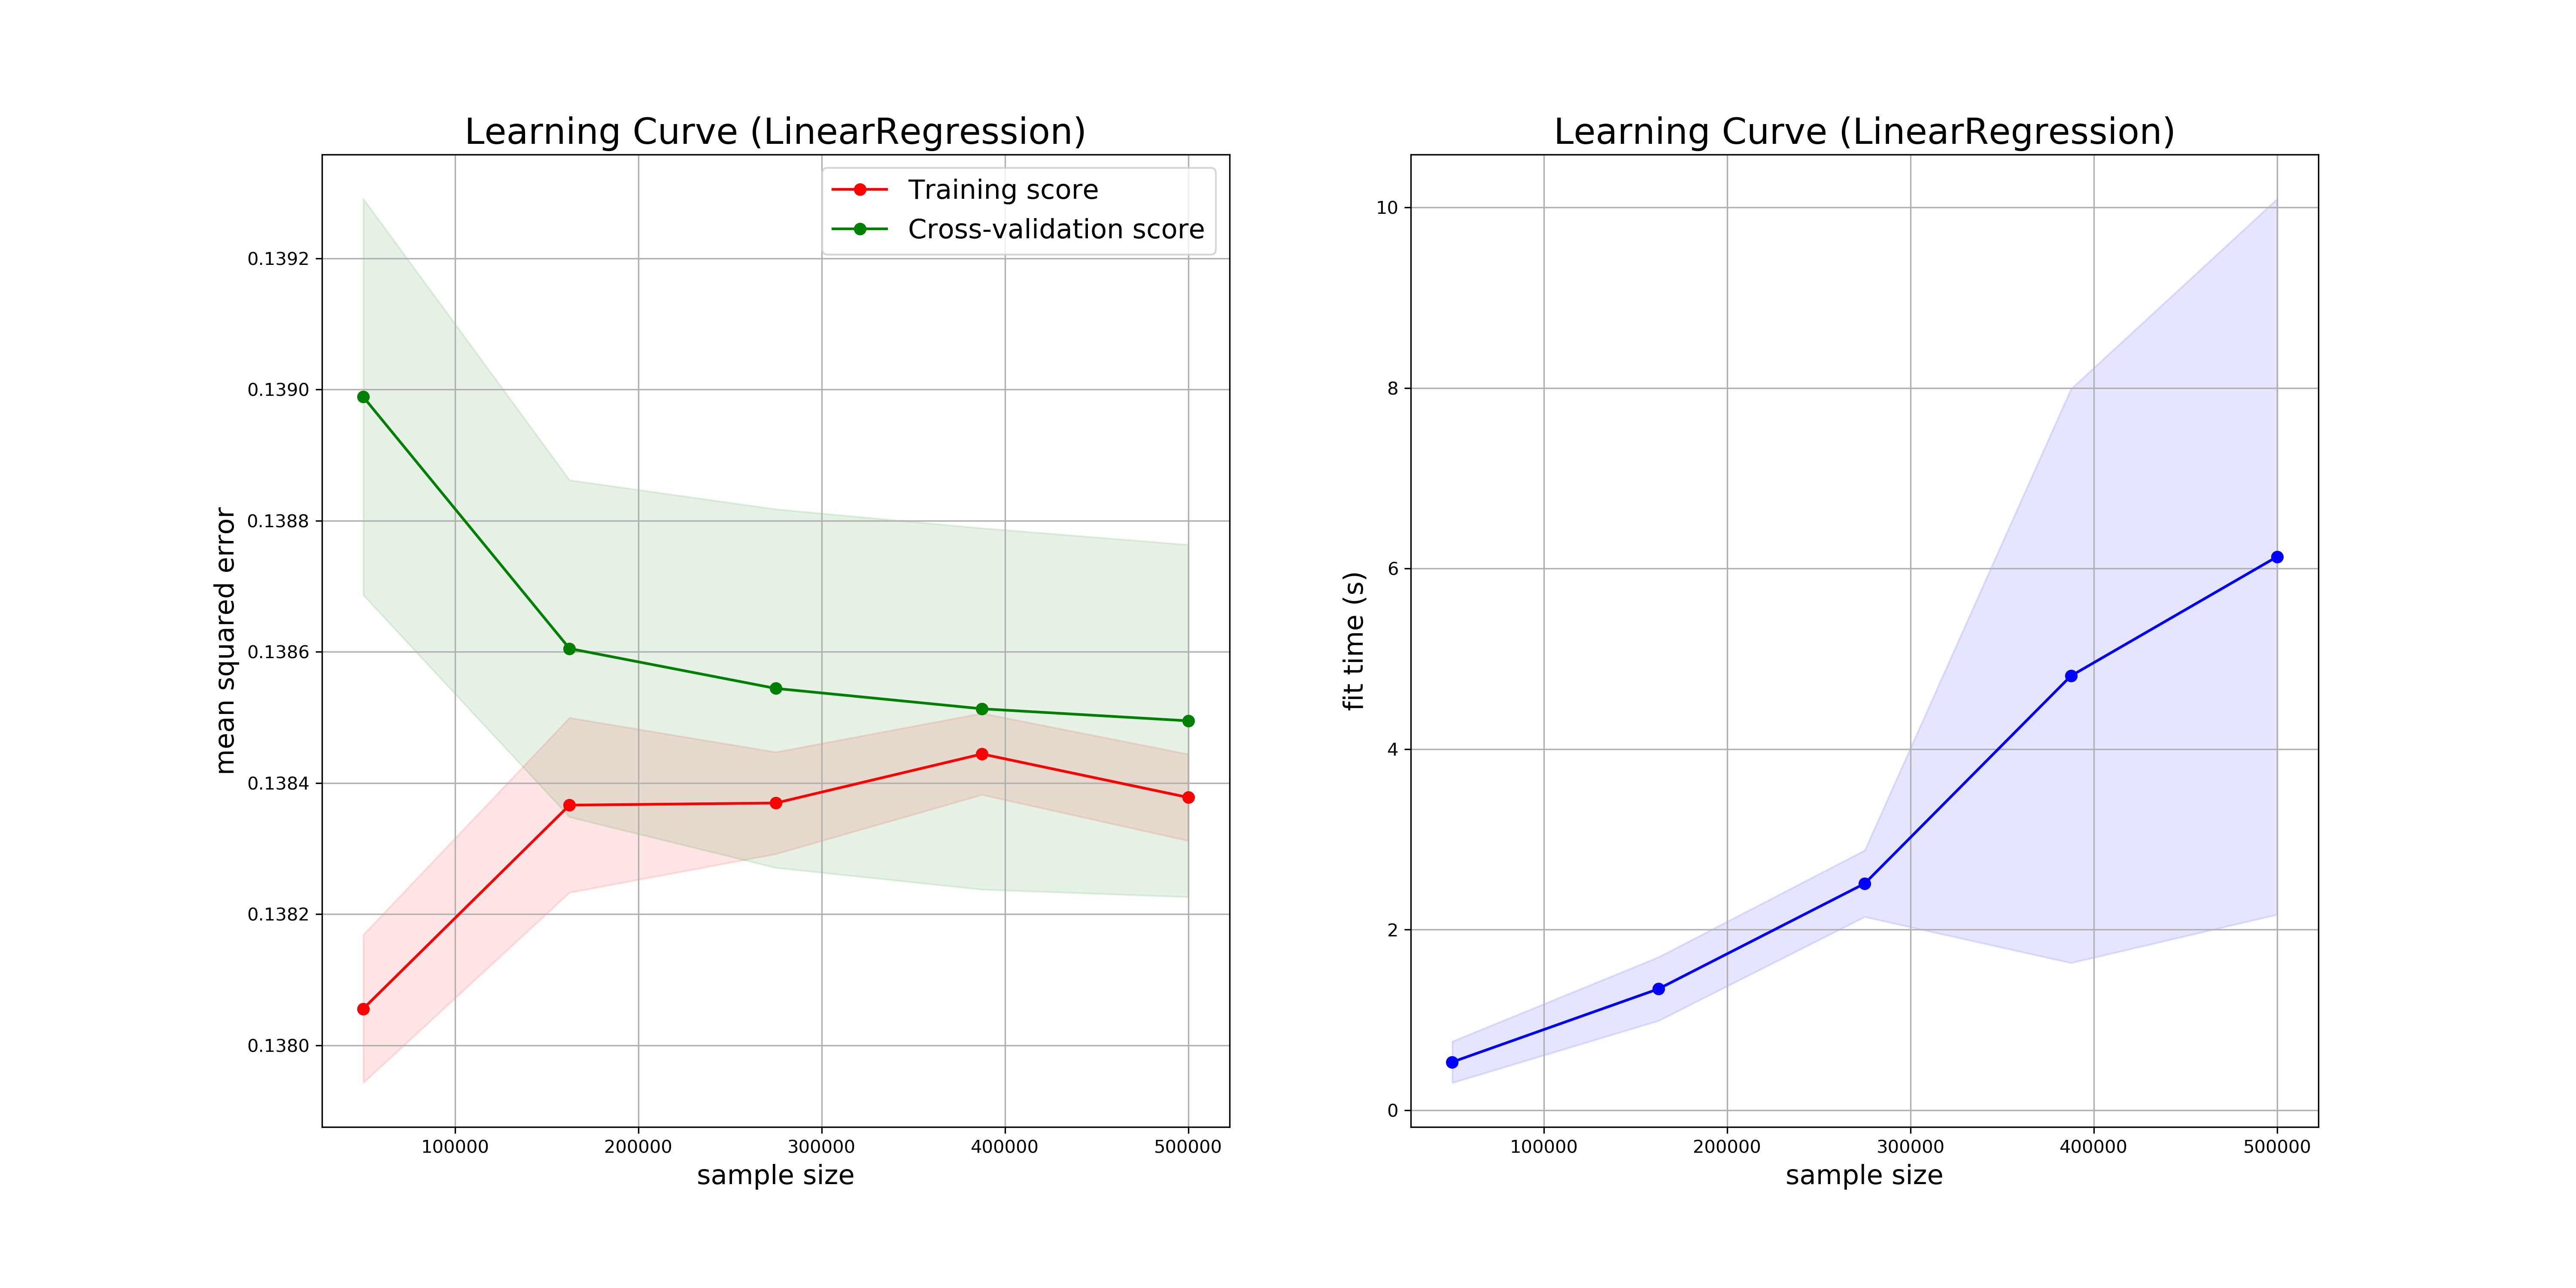
\includegraphics[width=0.7\textwidth]{linearregression-final.png}
\captionof{figure}{Linear Regression's learning curves(from left to right): Learning Curve For RMSE, Learning Curve For Time}
\label{fig:LR}

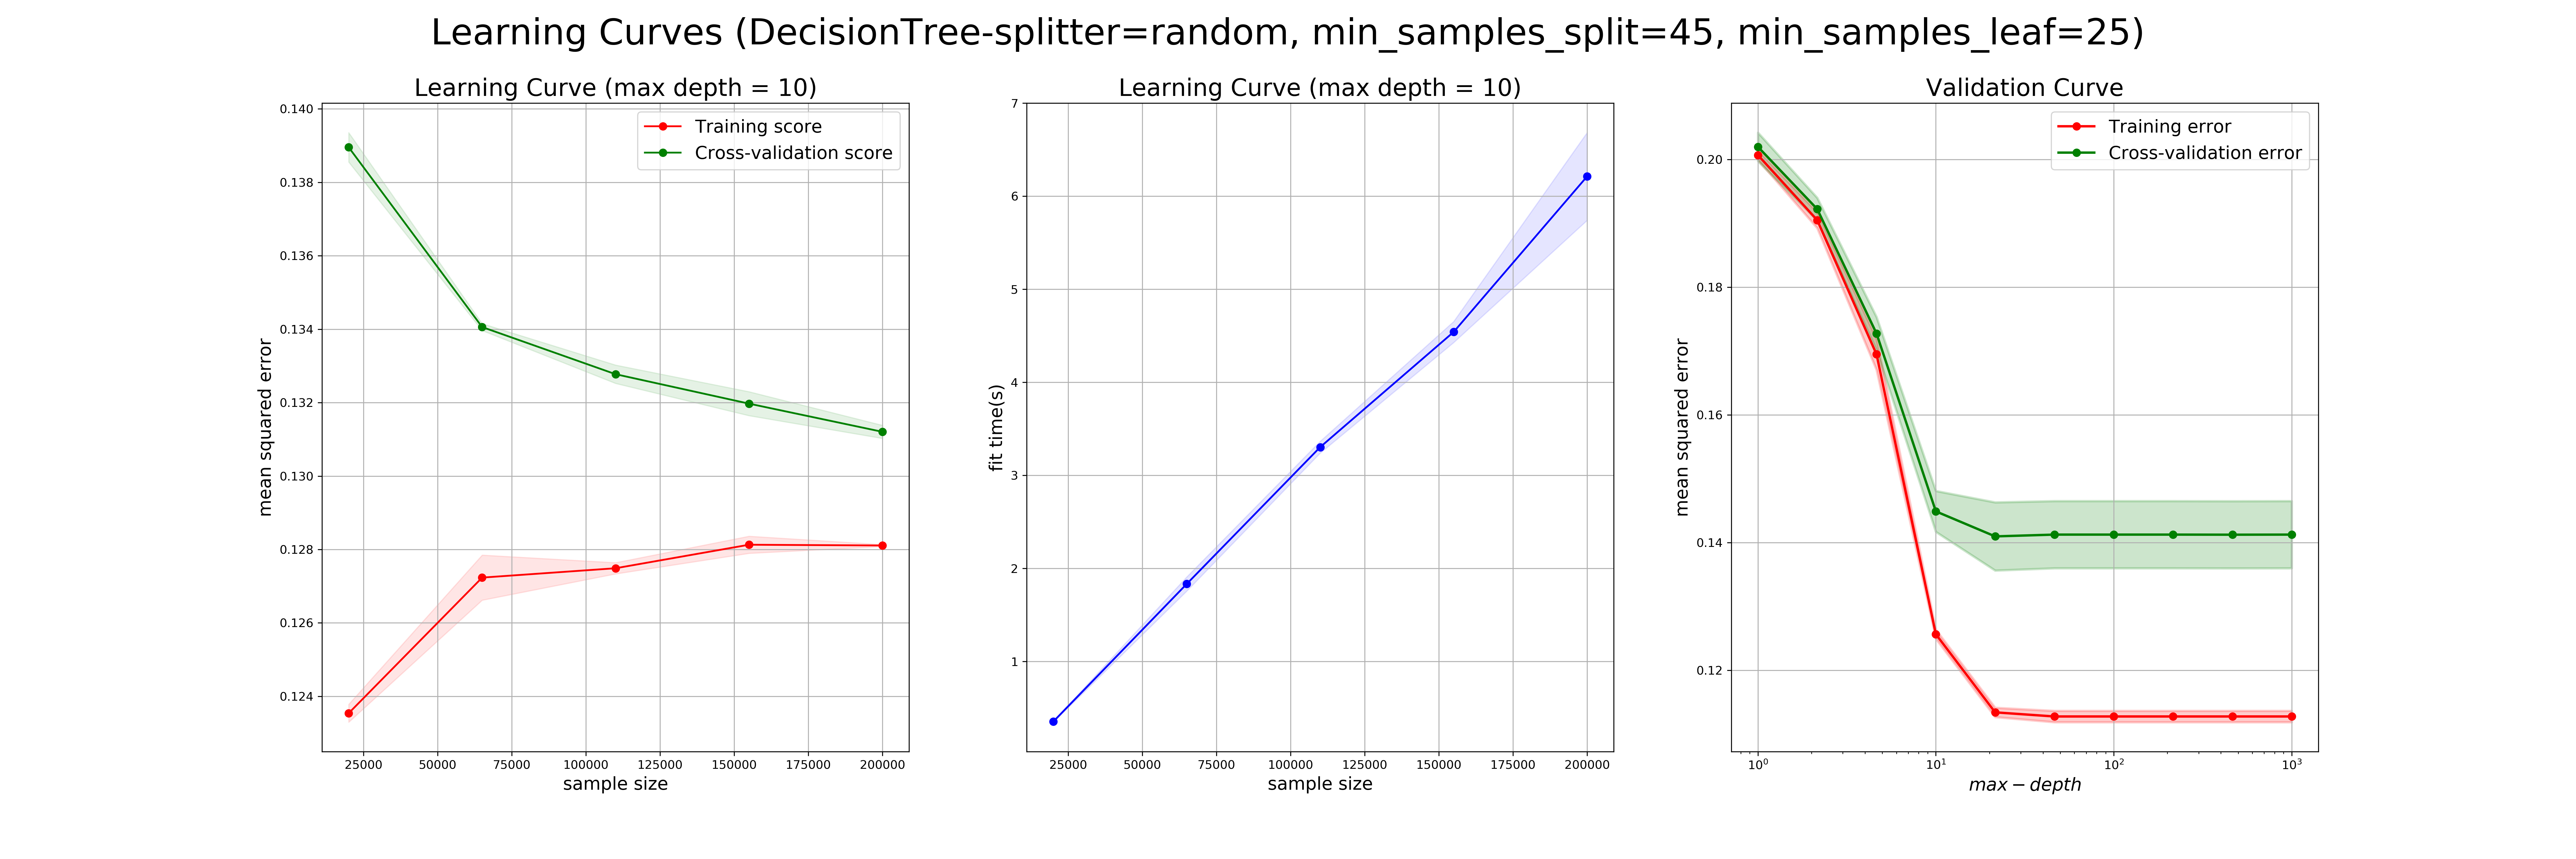
\includegraphics[width=1\textwidth]{decisiontree-final.png}
\captionof{figure}{Decision Tree's learning curves(from left to right): Learning Curve For RMSE, Learning Curve For Time, Cross Validation  Curve}
\label{fig:DT}

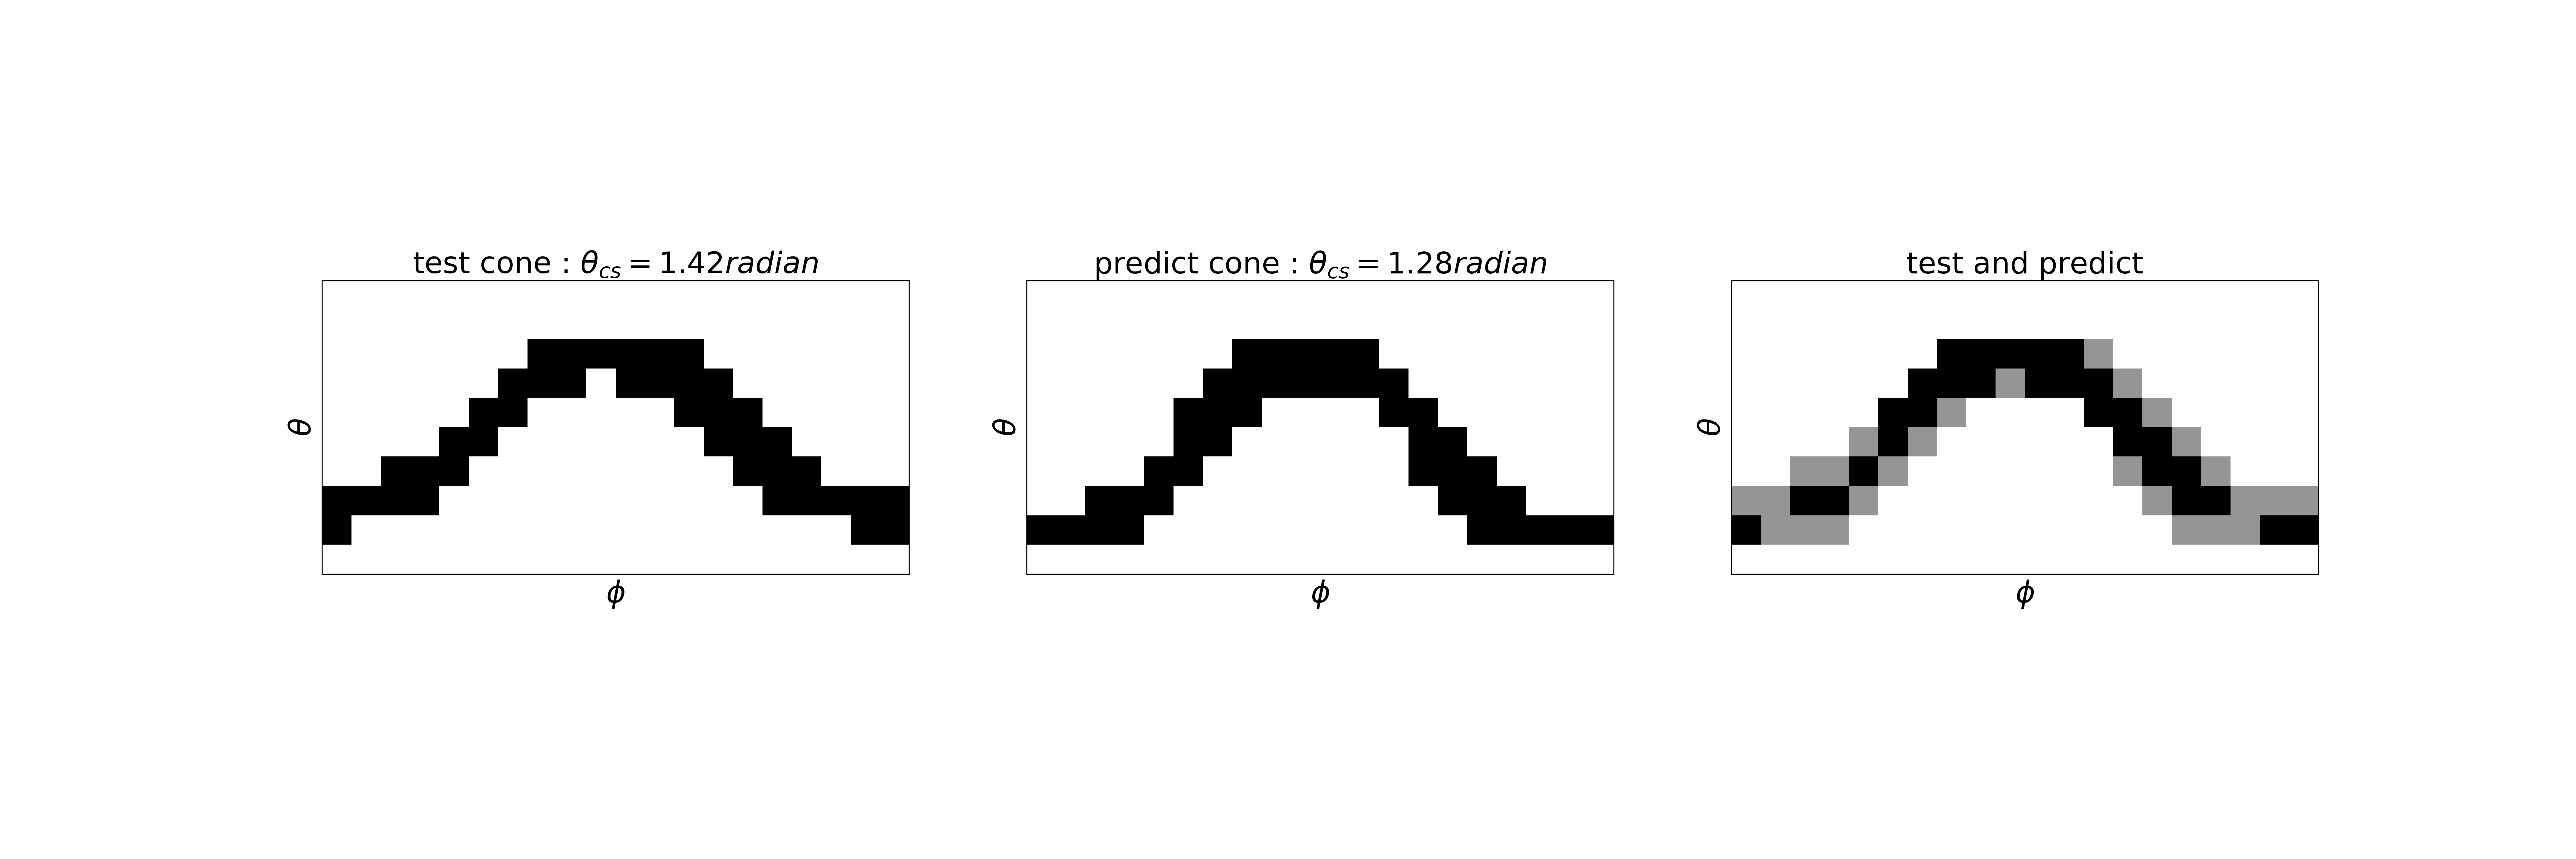
\includegraphics[width=1\textwidth]{cones.png}
\captionof{figure}{A cone-sphere intersection with $\theta_s$ predicted by KNN with error $RMSE\sim 0.018$}
\label{fig:cones}

\begin{table}[]
    \centering
\begin{tabular}{ c | c | c | c }
 Model & RMSE & Fit Time & Predict Time \\ 
 \hline
 SVR & 0.1257 & 8':35" & 8':34" \\  
 \hline
 KNN & 0.1044 & 1.26s & 12':38"\\
 \hline
 Kernel Ridge & 0.2331 & 35.9s & 9.11s\\
 \hline
 Linear Regression & 0.1387 & 5.83s & 2.12s\\
 \hline
 Decision Tree & 0.1314 & 8.07s & 826 ms
\end{tabular}
\caption{Final table of parameters that are crucial for finding the best estimator}
\label{table:final}
\end{table}


\begin{thebibliography}{99}
\bibitem{SVM}scikit-learn.org/stable/modules/svm.html
\bibitem{metric}medium.com/usf-msds/choosing-the-right-metric-for-machine-learning-models-part-1-a99d7d7414e4
\bibitem{alpha}scikit-learn.org/stable/modules/generated/sklearn.kernel\_ridge.KernelRidge.html
\end{thebibliography}
\end{document}
